\documentclass[11pt,letterpaper]{article}

\usepackage[margin=1in]{geometry}
\usepackage{parskip}
\usepackage{graphicx}
\usepackage{subcaption}
\usepackage{booktabs}
\usepackage{amsmath}
\usepackage{xcolor}
\usepackage{listings}
\usepackage{tikz}
\usetikzlibrary{positioning,arrows.meta,fit,backgrounds,calc}
\usepackage[superscript]{cite}
\usepackage[hidelinks]{hyperref}
\usepackage{url}

\definecolor{codebg}{gray}{0.96}
\definecolor{codekw}{RGB}{0,90,160}
\definecolor{codecomment}{RGB}{100,120,100}

\lstset{
  basicstyle=\ttfamily\footnotesize,
  backgroundcolor=\color{codebg},
  keywordstyle=\color{codekw},
  commentstyle=\color{codecomment},
  breaklines=true,
  frame=none,
  showstringspaces=false,
  columns=fullflexible,
  xleftmargin=6pt,
  aboveskip=6pt,
  belowskip=6pt,
}

\newcommand{\code}[1]{\texttt{\small #1}}

\title{Reproducing the Dragonblood WPA3/SAE Vulnerabilities\\
in a Containerized Virtual-Radio Laboratory}

\author{Vladimir Chukhlebov\\
University of Padua, Network Security\\
\texttt{vladimir.chukhlebov@studenti.unipd.it}}

\date{}

\begin{document}

\maketitle

\begin{abstract}
WPA3 replaced WPA2's Pre-Shared Key exchange with Simultaneous Authentication of
Equals (SAE), a password-authenticated key exchange built on the Dragonfly
handshake. In 2019 and 2020, Vanhoef and Ronen showed in their Dragonblood work
that SAE's password-to-group derivation leaks information through timing and
cache side channels, and that WPA3's transition mode can be downgraded to WPA2.
This paper documents a self-contained laboratory that reproduces three of those
findings: an SAE timing side channel, a WPA3 to WPA2 downgrade, and a full
password-recovery chain, all against a deliberately vulnerable
\code{hostap\_2\_4} access point. The lab runs entirely on virtual Wi-Fi radios
(\code{mac80211\_hwsim}) inside Docker containers, with a Lima VM providing the
Linux kernel on macOS, so no radio hardware is required. Following a three-phase
plan (software mock, emulation, physical hardware), we implement each attack
behind a common wireless-backend interface. We validate the attacks with 117
automated tests and confirm the timing leak statistically (Welch's t-test,
$p = 0.036$). The recovery step narrows a 100,000-word dictionary to a single
candidate using nine spoofed MAC addresses, recovering the target password. The
same recovery code was also run against a real and authorized home router; it
reported no usable timing signal, which is the expected result for current,
patched firmware. We also describe the main
practical problem, namely that sub-microsecond SAE computation made the timing
difference invisible in emulation, and its solution: a configurable per-iteration
delay added to hostapd.
\end{abstract}

\clearpage

\section{Introduction}

WPA3-Personal is the current consumer Wi-Fi security standard, and its central
improvement over WPA2 is the SAE handshake, which resists the offline dictionary
attacks that affect WPA2's four-way handshake. Because SAE is now the default on
new hardware, weaknesses in it matter more in practice than attacks on WPA2,
which is already known to be broken.

The Dragonblood work of Vanhoef and Ronen~\cite{vanhoef2020dragonblood} showed
that early SAE implementations leak password information through side channels
and that WPA3's backward-compatibility (transition) mode can be downgraded. This
project reproduces those results in a controlled, fully scripted environment, so
the attacks can be studied, tested, and re-run without physical Wi-Fi hardware
or a live target network.

Contributions:
\begin{itemize}
  \item A containerized WPA3 attack lab built on virtual radios
    (\code{mac80211\_hwsim}), runnable with a single \code{make up} command on
    Linux or macOS (via a Lima VM), targeting a pinned vulnerable hostapd.
  \item Three attacks implemented behind one wireless-backend interface: an SAE
    timing side channel, a WPA3 to WPA2 downgrade, and a multi-MAC
    timing-to-password recovery chain. The same recovery code runs against the
    emulated lab and, with the \code{live-recovery} tool, against a real AP.
  \item A statistical analysis pipeline (calibration, Welch's t-test, effect
    size, power analysis) with reproducible CSV, JSON, and figure output.
  \item A test suite of 117 automated tests across unit, integration, and full
    Docker end-to-end levels, and a plain account of the engineering problems
    encountered and how they were solved.
\end{itemize}

\section{Background: Dragonblood}
\label{sec:background}

\subsection{The SAE (Dragonfly) handshake}
SAE~\cite{ieee80211_2016,rfc7664} is a password-authenticated key exchange. Both
peers derive a shared secret element, the Password Element (PWE), from the
network password and their two MAC addresses, then exchange Commit frames
(containing a scalar and an elliptic-curve element) followed by Confirm frames
that prove knowledge of the derived key. Unlike WPA2, neither the password nor a
directly crackable hash is exposed on the wire, which is what makes SAE resistant
to offline dictionary attacks.

\subsection{Hash-to-curve and the hunting-and-pecking loop}
The vulnerable step is PWE derivation. For elliptic-curve groups, early SAE uses
a try-and-increment (hunting-and-pecking) loop: for counter = 1, 2, and so on, it
computes a candidate seed, HMAC-SHA256 of (MAC\_A, MAC\_B) keyed with (password,
counter), interprets it as an x-coordinate on the curve, and tests whether
$x^3 + ax + b$ is a quadratic residue modulo the field prime $p$. The loop stops
at the first counter that yields a valid point. Importantly, the number of
iterations depends on the password and the MAC pair. On the NIST P-256 curve
about half of all x values are valid, so the iteration count varies from password
to password~\cite{vanhoef2020dragonblood}. We reuse this exact computation later,
offline, to filter dictionary candidates.

\subsection{The timing side channel}
If the loop is not constant-time, the response latency of the AP correlates with
the iteration count, which in turn is a function of the password. An attacker who
sends SAE Commit frames from many different spoofed MAC addresses observes, for
each MAC, an iteration count for the (unknown) password. Vanhoef and Ronen report
that with fewer than 75 timing measurements per spoofed MAC address they can
recover the number of executed iterations~\cite{dragonblood_site}. The recovered
per-MAC iteration counts then act as a filter: any candidate password whose
computed iteration counts (which the attacker can calculate offline) disagree
with the observed counts is eliminated. Intersecting across enough MAC addresses
isolates the password.

\subsection{Other Dragonblood attack classes}
Beyond timing, Dragonblood~\cite{vanhoef2020dragonblood,dragonblood_site}
identifies cache-based side channels (memory-access patterns during PWE
derivation), transition-mode downgrade (a WPA3/WPA2 network pushed onto WPA2 by a
rogue AP), security-group downgrade via forged decline messages, and denial of
service, where as few as 16 forged commit frames per second drive high CPU load
on an AP. This project implements the timing side channel, its password-recovery
extension, and the transition-mode downgrade.

\subsection{Disclosure timeline and CVEs}
The initial disclosure was in April 2019. In August 2019 the Wi-Fi Alliance's
private mitigation (recommending Brainpool curves) was found to introduce a
second side channel; updated guidance followed in January 2020, and the full
paper appeared at IEEE S\&P 2020~\cite{vanhoef2020dragonblood}. Relevant
identifiers include CVE-2019-9494 (SAE side channels)~\cite{cve_2019_9494},
CVE-2019-13377 (Brainpool timing)~\cite{cve_2019_13377}, and the EAP-pwd family
such as CVE-2019-9497~\cite{cve_2019_9497}.

\section{Threat Model and Scope}
The attacker is within radio range of the target AP, can transmit and receive
802.11 management and authentication frames, and can spoof arbitrary source MAC
addresses, but does not know the password. The target is a pinned, pre-patch
build of hostapd (the \code{hostap\_2\_4} release tag, from before the
constant-time Dragonblood fixes), configured for WPA3-SAE on NIST P-256
(group 19). This mirrors the deployed embedded devices that motivated the
original research. Modern, patched APs use constant-time PWE derivation, so the
lab targets the historical vulnerable behavior, not current firmware.

\section{Implementation Plan and Phases}
\label{sec:phases}
The project was structured as a three-phase progression, where each phase
reduces uncertainty before adding real-world complexity:

\begin{enumerate}
  \item \textbf{Mock phase.} The attack logic (frame construction, timing
    collection, calibration, statistics, dictionary filtering) is exercised
    against an in-process model of a vulnerable SAE responder
    (\code{VulnerableMockBackend}), which computes the true iteration count for a
    password and MAC pair and returns a modeled response time. This checks
    correctness with no hardware or containers.
  \item \textbf{Emulation phase.} The same attack code runs unchanged against a
    real hostapd, over virtual radios provided by the Linux
    \code{mac80211\_hwsim} kernel module, inside Docker containers.
  \item \textbf{Physical phase.} Reproduction against real Wi-Fi hardware to
    confirm the emulation findings, done with the \code{live-recovery} tool
    (Section~\ref{sec:results}).
\end{enumerate}

The key enabler is a single interface, \code{WirelessBackend}, with concrete
implementations for the mock, and for real or emulated interfaces via Scapy.
Attack modules depend only on this interface, so moving from mock to emulation to
hardware does not change a line of attack logic; only the injected backend
changes. The physical phase follows directly from this design:
\code{live-recovery} runs the same recovery attack against a real access point,
adding only what a live target needs (monitor-mode setup, channel discovery, and
a verdict), rather than reimplementing anything.

\section{System Architecture}
\label{sec:architecture}

\begin{figure}[ht]
  \centering
  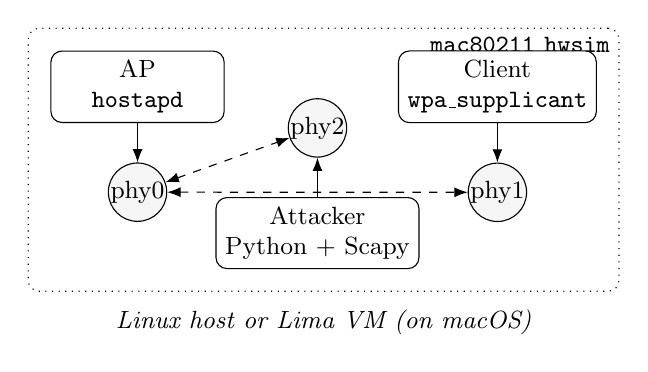
\begin{tikzpicture}[
      font=\small,
      box/.style={draw, rounded corners, minimum height=8mm, minimum width=22mm,
                  align=center, fill=white},
      radio/.style={draw, circle, minimum size=6mm, inner sep=0pt, fill=codebg},
      >=Latex,
    ]
    \node[box] (ap) {AP\\\code{hostapd}};
    \node[box, right=22mm of ap] (cl) {Client\\\code{wpa\_supplicant}};
    \node[box, below=14mm of $(ap)!0.5!(cl)$] (att) {Attacker\\Python + Scapy};

    \node[radio, below=5mm of ap] (r0) {phy0};
    \node[radio, below=5mm of cl] (r1) {phy1};
    \node[radio, above=5mm of att] (r2) {phy2};

    \draw[->] (ap) -- (r0);
    \draw[->] (cl) -- (r1);
    \draw[->] (att) -- (r2);
    \draw[<->, dashed] (r0) -- (r1);
    \draw[<->, dashed] (r0) -- (r2);

    \begin{scope}[on background layer]
      \node[draw, dotted, rounded corners, fit=(ap)(cl)(att)(r0)(r1)(r2),
            inner sep=8pt,
            label={[anchor=north east]north east:\code{mac80211\_hwsim}}] (host) {};
    \end{scope}
    \node[below=1mm of host.south, font=\small\itshape]
      {Linux host or Lima VM (on macOS)};
  \end{tikzpicture}
  \caption{Lab topology. Three containers (AP, Client, Attacker) each own a
  virtual radio created by \code{mac80211\_hwsim}; frames travel through the
  kernel rather than the air. On macOS a Lima VM supplies the Linux kernel.}
  \label{fig:arch}
\end{figure}

\subsection{Containers and virtual radios}
The lab (Figure~\ref{fig:arch}) has three Docker containers: an \textbf{AP}
running the vulnerable hostapd, a \textbf{Client} running \code{wpa\_supplicant}
(used to establish a legitimate SAE baseline), and an \textbf{Attacker} running
the Python and Scapy attack tools. The AP and Client use \code{network\_mode:
none}; the Attacker uses host networking for notebook access. All run privileged
with \code{pid: host} so they can manage wireless interfaces. The
\code{mac80211\_hwsim} module~\cite{mac80211_hwsim} creates three virtual PHYs on
the host; \code{host/setup.sh} loads the module and \code{host/assign-phys.sh}
moves each PHY into a container's network namespace. Because frames pass through
the kernel instead of the air, the channel is noise free and deterministic. As
Section~\ref{sec:problems} explains, that property also removed the timing
difference the attacks rely on.

\subsection{macOS support via Lima}
\code{mac80211\_hwsim} is a Linux kernel module and is not available on macOS. A
Lima VM (\code{lima/wifi-lab.yaml}) provides an Ubuntu guest with Docker and the
wireless stack; the \code{Makefile} detects the OS and forwards every target into
the VM via \code{host/vm-exec.sh}, so the developer experience is the same on
both platforms.

\subsection{Image hierarchy and configuration}
A four-layer Docker build keeps images small and cache friendly:
\code{wifi-lab-base}, then \code{wifi-lab-builder} (hostap source and build
dependencies), then the AP and Client (compile plus runtime). The Attacker image
extends the base directly. Attack-specific infrastructure changes, such as
putting the AP into transition mode for the downgrade experiment, are layered as
Compose overlays (\code{docker-compose.downgrade.yml}) rather than duplicated
images. Configuration files (\code{hostapd\_sae.conf}, its transition variant,
and \code{wpa\_supplicant\_sae.conf}) are bind-mounted, not baked in.

\subsection{Attack framework}
Every attack shares one lifecycle: reconnaissance, execution, then analysis.
Reconnaissance scans for the target AP; execution collects the raw timing or
capture data; analysis runs the statistics and writes the report. Configuration
is passed as typed, immutable objects rather than loose dictionaries. Each run
writes a timestamped directory under \code{results/} containing the raw samples
(CSV), the analysis report (JSON), run metadata, and plots, so every result in
this paper is reproducible from committed artifacts.

\section{Implementation Walkthrough}
Bringing up the lab and running an attack is a short sequence:
\begin{enumerate}
  \item \code{make up}: on macOS, start the Lima VM, load
    \code{mac80211\_hwsim}, build the images, launch the three containers, and
    assign the virtual PHYs to their namespaces.
  \item The AP loads \code{hostapd\_sae.conf} (SSID \code{DragonbloodLab},
    \code{wpa\_key\_mgmt=SAE}, PMF required, channel 6); the Client associates
    over SAE to confirm a working WPA3 network.
  \item \code{make attack-timing}, \code{attack-downgrade}, or
    \code{attack-recovery} resolves the AP's BSSID and runs the matching CLI
    entry point inside the Attacker container, writing artifacts to
    \code{results/}.
\end{enumerate}
The three CLI entry points (\code{timing-attack}, \code{downgrade-attack},
\code{recovery-attack}) are declared in \code{pyproject.toml}. Each accepts the
shared arguments \code{-{}-interface}, \code{-{}-bssid}, \code{-{}-ssid},
\code{-{}-channel}, and \code{-{}-output-dir}.

\section{Attacks and Results}
\label{sec:results}
All results below are the reference runs committed under \code{results/}
(netem profile: clean).

\subsection{SAE timing side channel}
The timing side-channel attack measures the AP's SAE Commit response time for
several password groups. For each group it repeatedly resets AP state with a
deauthentication, sends a freshly crafted SAE Commit frame, and records the
round-trip latency at nanosecond resolution. It then computes per-group
descriptive statistics and runs pairwise Welch's t-tests (unequal variance,
$\alpha = 0.05$).

Table~\ref{tab:timing} reports the reference run (ten samples per group). The
mean response time is highest for the short group (46.8 ms) and lower for medium
(42.0 ms) and long (44.0 ms). The short-versus-medium difference is
statistically significant ($p = 0.036$); the other pairs are not, at this small
sample size. Figures~\ref{fig:timing-box} and~\ref{fig:timing-hist} show the
distributions. The significant pair confirms that the emulated AP's SAE timing is
password-dependent, so the side channel is present and detectable. The absolute
latencies here reflect the per-iteration delay configured for this run; only the
relative differences between groups matter.

\begin{table}[ht]
  \centering
  \caption{SAE timing side channel: per-group statistics and pairwise Welch's
  t-tests (10 samples per group).}
  \label{tab:timing}
  \begin{tabular}{lccc}
    \toprule
    Password group & Mean (ms) & Median (ms) & Std (ms) \\
    \midrule
    short  & 46.8 & 45.5 & 5.40 \\
    medium & 42.0 & 42.3 & 3.97 \\
    long   & 44.0 & 42.9 & 4.55 \\
    \midrule
    Comparison & \multicolumn{2}{c}{p-value} & Significant \\
    \midrule
    short vs medium & \multicolumn{2}{c}{0.036} & yes \\
    short vs long   & \multicolumn{2}{c}{0.220} & no  \\
    medium vs long  & \multicolumn{2}{c}{0.314} & no  \\
    \bottomrule
  \end{tabular}
\end{table}

\begin{figure}[ht]
  \centering
  \begin{subfigure}{0.49\textwidth}
    \centering
    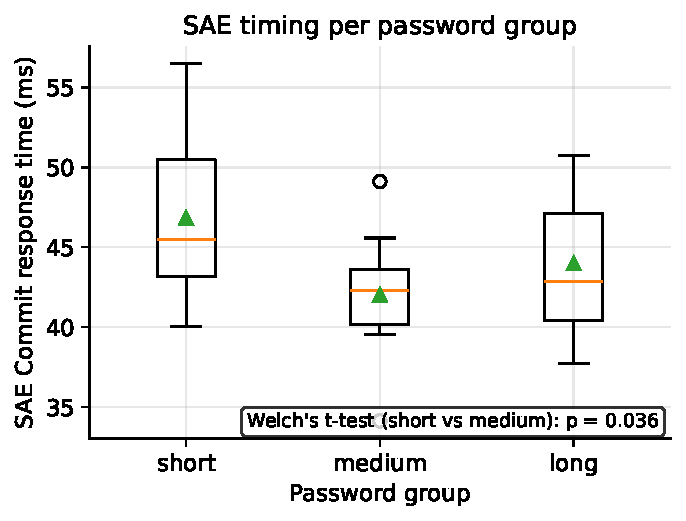
\includegraphics[width=\linewidth]{figures/timing_boxplot.pdf}
    \caption{Response-time distribution per group.}
    \label{fig:timing-box}
  \end{subfigure}\hfill
  \begin{subfigure}{0.49\textwidth}
    \centering
    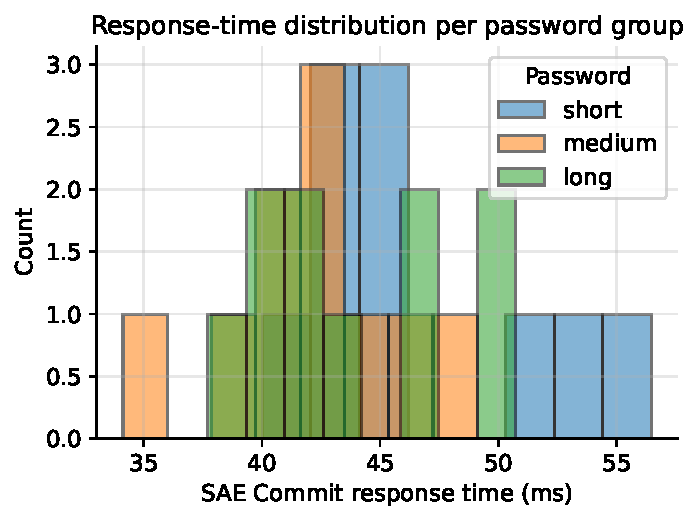
\includegraphics[width=\linewidth]{figures/timing_hist.pdf}
    \caption{Overlaid response-time histograms.}
    \label{fig:timing-hist}
  \end{subfigure}
  \caption{SAE Commit response times per password group. The short group is
  slower, consistent with a larger hash-to-curve iteration count.}
  \label{fig:timing}
\end{figure}

\subsection{Password recovery via multi-MAC intersection}
The password-recovery attack turns the timing leak into an actual password. It
collects SAE Commit timings from up to 15 spoofed source MAC addresses, 200
samples each in the reference run, then does two things:

\begin{enumerate}
  \item \textbf{Calibrates.} The calibration step takes the mean response time
    per MAC, sets the baseline to the smallest mean, and finds the per-iteration
    time $\Delta t$ as the smallest gap between sorted means that exceeds a noise
    threshold of three times the average standard error. The estimated iteration
    count for a MAC is $\mathrm{round}((\mathrm{mean} - \mathrm{baseline}) /
    \Delta t) + 1$. The reference run calibrated to a baseline of about
    499~$\mu$s, a $\Delta t$ of about 491~$\mu$s, and six distinct clusters
    (Figure~\ref{fig:clusters}).
  \item \textbf{Filters.} Starting from the full 100,000-word dictionary, it
    computes each candidate's true iteration count for each MAC offline and keeps
    only candidates whose computed count matches the observed one. Intersecting
    across MACs shrinks the candidate set monotonically.
\end{enumerate}

Table~\ref{tab:recovery} and Figure~\ref{fig:narrowing} show the narrowing:
after nine MAC addresses the 100,000-word dictionary collapses to a single
candidate, and the attack recovers the target password (\code{dr4gonfly}). This
is the main result: a correct password, embedded in a large dictionary,
extracted purely from response-time statistics.

\begin{table}[ht]
  \centering
  \caption{Password recovery: per-MAC estimated iteration count and the
  remaining candidate set after intersecting each MAC.}
  \label{tab:recovery}
  \begin{tabular}{clr}
    \toprule
    MAC (last byte) & Est.\ iterations & Candidates remaining \\
    \midrule
    \code{:00} & 1 & 49,853 \\
    \code{:01} & 3 & 6,341 \\
    \code{:02} & 1 & 3,212 \\
    \code{:03} & 1 & 1,615 \\
    \code{:04} & 2 & 444 \\
    \code{:05} & 1 & 238 \\
    \code{:06} & 1 & 111 \\
    \code{:07} & 5 & 2 \\
    \code{:08} & 2 & \textbf{1} \\
    \bottomrule
  \end{tabular}
\end{table}

\begin{figure}[ht]
  \centering
  \begin{subfigure}{0.49\textwidth}
    \centering
    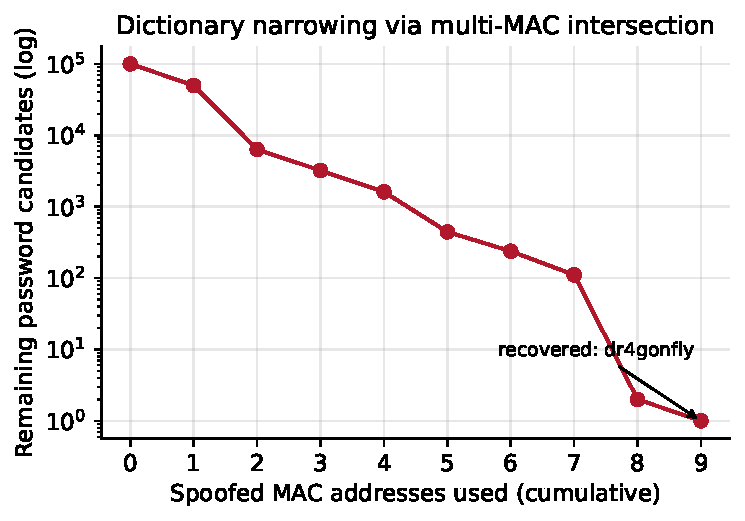
\includegraphics[width=\linewidth]{figures/recovery_narrowing.pdf}
    \caption{Candidate narrowing (log scale).}
    \label{fig:narrowing}
  \end{subfigure}\hfill
  \begin{subfigure}{0.49\textwidth}
    \centering
    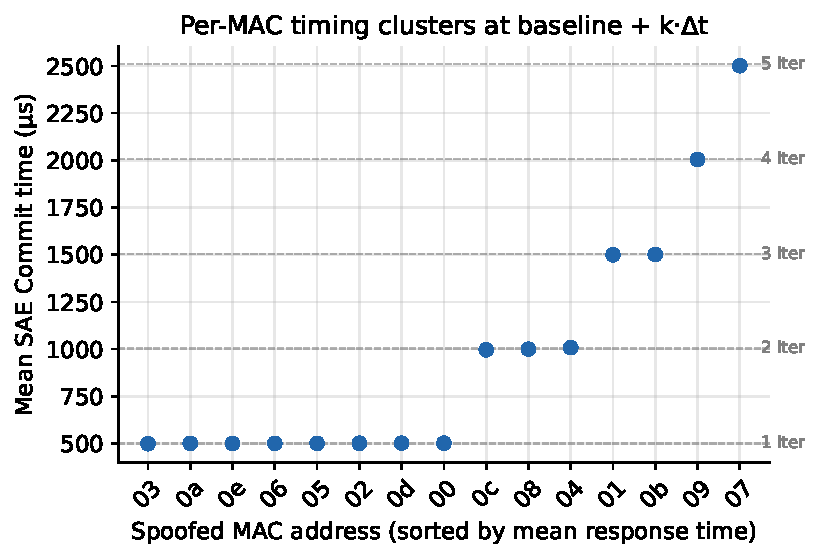
\includegraphics[width=\linewidth]{figures/recovery_clusters.pdf}
    \caption{Per-MAC mean time, by iteration count.}
    \label{fig:clusters}
  \end{subfigure}
  \caption{Password recovery. (a) Nine spoofed MACs reduce 100,000 candidates to
  one. (b) Per-MAC means cluster at $\mathrm{baseline} + k\,\Delta t$ for integer
  $k$, the structure the calibrator uses.}
  \label{fig:recovery}
\end{figure}

\subsection{WPA3 to WPA2 downgrade}
The downgrade attack targets WPA3 transition mode, in which an AP advertises both
SAE and WPA2-PSK for backward compatibility. The attack forges beacons for the
same SSID whose RSN Information Element advertises only WPA2-PSK, built by
stripping the SAE AKM suite (00-0F-AC:8) and leaving PSK (00-0F-AC:2). A background sniffer watches for a resulting WPA2 four-way
handshake, which would indicate the client downgraded and can then be attacked
with classic offline WPA2 techniques.

In the reference run the attacker injected 71 forged beacons over five seconds
and captured zero WPA2 handshakes: the emulated client did not downgrade. We
report this outcome plainly. It reflects the emulated client's configuration (the
Client is set to require SAE, so it correctly refuses WPA2), not a flaw in the
forging logic, which unit tests confirm produces a well-formed WPA2-only RSN IE.
The mechanism and its success condition (a captured handshake) are the
contribution here; chaining a successful downgrade into a full WPA2 compromise
(for example KRACK or a dictionary attack on the captured handshake) is left as
future work.

\subsection{Physical phase: field test against a real router}
\label{sec:field}
To move from emulation to hardware we built \code{live-recovery}, a command-line
tool that runs the same recovery attack against a real access point. Over the
emulated version it adds only what a live target requires: enabling monitor mode,
sweeping channels to discover the AP, and mapping the result to a plain verdict,
one of \code{vulnerable-recovered}, \code{vulnerable-partial},
\code{patched-no-signal}, or \code{target-not-found}. The "no signal" case is
detected precisely: calibration reports no signal when every per-MAC mean falls
within the noise floor, which is the signature of a constant-time PWE derivation.

We ran it against the author's own and authorized home router, a WPA2/WPA3
transition-mode access point. The calibrator found no per-iteration timing signal
above noise, so the tool reported \code{patched-no-signal}: no usable side
channel. This is the expected and correct outcome for current firmware, whose SAE
derivation is constant-time. The negative result is useful on two counts: it
confirms that the deployed Dragonblood mitigation is effective, and it shows that
the calibration step does not report a signal that is not there (no false
positive). A positive field result would require a known-vulnerable legacy
device.

\section{Problems Encountered and Solutions}
\label{sec:problems}

\subsection{Sub-microsecond SAE made timing invisible}
The main problem: in emulation, \code{mac80211\_hwsim} passes frames through the
kernel with no radio latency, and hostapd's PWE derivation on a modern CPU
completes in well under a $\mu$s per iteration. The per-iteration timing signal
was therefore far below measurement noise, so the effect the attack relies on
could not be measured.

The solution was to make the iteration cost explicit and adjustable by patching
hostapd to sleep a configurable interval after each hash-to-curve iteration
(Listing~\ref{lst:patch}). The delay is read once from the
\code{SAE\_ITERATION\_DELAY\_US} environment variable (default 3000~$\mu$s, that
is 3~ms) and applied inside hostapd's PWE-derivation loop. This models the slower
PWE derivation of the embedded devices Dragonblood targeted, and it changes only
the size of the per-iteration cost, not the attack logic, which is identical to
what would run against real hardware. We set the default to 3~ms from the
emulation's own jitter: the timing run's standard deviation is about 4.5~ms, so
with 200 samples per MAC the calibration threshold is about 1~ms. A 3~ms delay
therefore clears the noise floor with margin, while 1~ms would sit on it.

\begin{lstlisting}[caption={The per-iteration timing delay added to hostapd's
SAE PWE derivation (\code{timing\_delay.patch}).},
label={lst:patch}]
@@ src/common/sae.c: sae_derive_pwe_ecc()
   if (hmac_sha256_vector(addrs, sizeof(addrs), 2,
                          addr, len, pwd_seed) < 0)
       break;
+  {
+      static int delay_us = -1;
+      if (delay_us < 0) {
+          const char *env =
+              getenv("SAE_ITERATION_DELAY_US");
+          delay_us = env ? atoi(env) : 3000;
+      }
+      usleep(delay_us);
+  }
   res = sae_test_pwd_seed_ecc(sae, pwd_seed, ...);
\end{lstlisting}

\subsection{Noise and discrete iteration counts}
Even with an amplified signal, individual measurements are noisy. Rather than
trusting single samples, the calibrator works on per-MAC means and uses the fact
that true iteration counts are integers: means cluster at
$\mathrm{baseline} + k\,\Delta t$ for integer $k$ (Figure~\ref{fig:clusters}). A
$3\sigma$-style noise threshold separates genuine gaps between clusters from
jitter, and a validation step warns if larger gaps are not clean integer
multiples of $\Delta t$.

\subsection{macOS has no \code{mac80211\_hwsim}}
As noted in Section~\ref{sec:architecture}, this was solved with a Lima VM and
Makefile forwarding, so the lab is a single command on both Linux and macOS.

\subsection{Reproducibility versus realism}
For deterministic tests the password is fixed (\code{dr4gonfly}) across the AP
config and the recovery assertions. This ties tests to a known value, a
deliberate trade-off that favors reproducible, checkable end-to-end runs over
realism; the attack itself makes no use of the known password.

\subsection{Physical phase}
For the physical phase we built \code{live-recovery} (Section~\ref{sec:field}),
which runs the same recovery attack against a real access point, adding
monitor-mode setup, channel discovery, and a verdict. Run against the author's
own patched home router, it recovered nothing
and reported \code{patched-no-signal}, the expected result, since current
firmware derives the password element in constant time. This is not a failure: it
confirms the deployed fixes work and that the tool does not produce false
positives. One caveat surfaced during this work: the default channel sweep covers
2.4 GHz (channels 1, 6, 11), so 5 GHz targets such as the test router require an
explicit \code{-{}-channel} (or \code{-{}-channels}).

\section{Testing and Validation}
The lab is covered by 117 automated tests (Table~\ref{tab:tests}), organized as a
pyramid. Unit tests (75) cover pure logic: SAE and RSN frame construction, the
statistics and calibration math, plotting, and channel discovery. Integration
tests (20) drive full attack pipelines against the mock backend, including the
end-to-end recovery of \code{dr4gonfly} from a small dictionary and the
\code{live-recovery} tool (vulnerable, patched, and target-not-found verdicts). End-to-end tests (22) stand up the actual Docker lab over
\code{mac80211\_hwsim} and check real SAE association, attack exit codes, and the
presence and shape of the CSV, JSON, and plot artifacts.

\begin{table}[ht]
  \centering
  \caption{Automated test suite (117 tests total).}
  \label{tab:tests}
  \begin{tabular}{llc}
    \toprule
    Level & Scope & Count \\
    \midrule
    Unit        & frame/RSN/crypto, stats, calibration, discovery & 75 \\
    Integration & mock-backend and live-recovery pipelines         & 20 \\
    End-to-end  & full Docker lab over \code{mac80211\_hwsim}      & 22 \\
    \midrule
    \multicolumn{2}{l}{\textbf{Total}} & \textbf{117} \\
    \bottomrule
  \end{tabular}
\end{table}

\section{Limitations and Future Work}
\label{sec:future}
The lab targets NIST P-256 (group 19) only; Brainpool and MODP groups, which show
their own timing behavior~\cite{cve_2019_13377}, are not yet modeled. The timing
signal is amplified by an injected delay; while the attack logic is identical to
a hardware attack, absolute latencies are not representative of a specific device.
Physical validation against a known-vulnerable device is still open: the only
accessible real AP was patched (the expected modern case), so the field test
correctly returned no signal. A natural next step is to buy several of the
cheapest popular WPA3 routers on Amazon or Alibaba, which often ship outdated
firmware, and test them for the timing side channel. Also open are completing the
downgrade-to-WPA2 attack chain (capturing and cracking a real four-way handshake,
or chaining KRACK) and a 5 GHz-aware default channel sweep. The design is
extensible, so FragAttacks and cache side channels are natural next targets.

\section{Conclusion}
We reproduced three Dragonblood results, an SAE timing side channel, a
transition-mode downgrade, and a full timing-to-password recovery, in a scripted,
hardware-free lab built on virtual radios and a pinned vulnerable hostapd. The
recovery step extracted a correct password from a 100,000-word dictionary using
nine spoofed MAC addresses, and the timing leak was confirmed statistically. The
main lesson is that emulation's determinism removes the very timing signal these
attacks rely on, and that a small, configurable delay in PWE derivation restores
an observable and faithful side channel without changing the attack. The result
is a reproducible platform for studying WPA3's weaknesses and, by extension, the
value of the constant-time fixes now deployed.

\clearpage
\appendix
\section{Reproducibility}
\label{sec:repro}
\noindent\textbf{Prerequisites.} Docker and \code{make}. On macOS, Lima
(\code{brew install lima}); the \code{Makefile} detects the OS and runs the Linux
steps inside the VM.

\noindent\textbf{Bring up the lab.}
\begin{lstlisting}[language=bash]
make up      # VM (macOS) + load mac80211_hwsim +
             # build images + start AP/Client/Attacker
make test    # verify SAE association (AP and Client)
\end{lstlisting}

\noindent\textbf{Run the attacks.} Artifacts are written to
\code{results/<attack>/<timestamp>/} (\code{raw\_samples.csv},
\code{analysis.json}, \code{metadata.json}, \code{plots/}):
\begin{lstlisting}[language=bash]
make attack-timing      # SAE timing side channel
make attack-downgrade   # WPA3 to WPA2 downgrade
make attack-recovery    # timing to password recovery
\end{lstlisting}

\noindent\textbf{Physical (live) target.} Against a real and authorized AP, on a
Linux host with a monitor-capable adapter:
\begin{lstlisting}[language=bash]
sudo make attack-live IFACE=wlan0 SSID='HomeWiFi' \
  DICT=/path/wordlist.txt
# 5 GHz targets: add --channel <n> (default sweep is 2.4 GHz)
\end{lstlisting}
The verdict is one of vulnerable-recovered, vulnerable-partial,
patched-no-signal, or target-not-found.

\noindent\textbf{Tuning and hardware-free runs.} The timing amplitude is set by
\code{SAE\_ITERATION\_DELAY\_US} (default 3000). Any attack accepts
\code{-{}-dry-run} to use the in-process modeling backend, so no lab is required.

\noindent\textbf{Tests.}
\begin{lstlisting}[language=bash]
make test-unit   # unit + integration (local, no VM)
make test-e2e    # brings up the lab, runs all e2e tests
\end{lstlisting}

\noindent\textbf{Rebuilding this paper.} Run \code{docs/paper/build.sh}, which
regenerates the figures from \code{results/} and compiles \code{paper.tex}.

\clearpage
\begin{thebibliography}{9}

\bibitem{vanhoef2020dragonblood}
M.~Vanhoef and E.~Ronen, "Dragonblood: Analyzing the Dragonfly handshake of
WPA3 and EAP-pwd," in \emph{2020 IEEE Symp.\ on Security and Privacy (S\&P)},
2020, pp.\ 517-533.

\bibitem{dragonblood_site}
M.~Vanhoef and E.~Ronen, "Dragonblood: Analysing WPA3's Dragonfly handshake,"
2019. Available: \url{https://wpa3.mathyvanhoef.com/}

\bibitem{cve_2019_9494}
MITRE, "CVE-2019-9494: SAE side-channel attacks (Dragonblood)," 2019.
Available: \url{https://cve.mitre.org/cgi-bin/cvename.cgi?name=CVE-2019-9494}

\bibitem{cve_2019_13377}
MITRE, "CVE-2019-13377: Timing side-channel in WPA3 SAE with Brainpool
curves," 2019. Available:
\url{https://cve.mitre.org/cgi-bin/cvename.cgi?name=CVE-2019-13377}

\bibitem{cve_2019_9497}
MITRE, "CVE-2019-9497: EAP-pwd reflection and side-channel attacks," 2019.
Available: \url{https://cve.mitre.org/cgi-bin/cvename.cgi?name=CVE-2019-9497}

\bibitem{ieee80211_2016}
IEEE, \emph{IEEE Std 802.11-2016}, Sec.\ 12.4 (Authentication using a password,
SAE), 2016.

\bibitem{rfc7664}
D.~Harkins, "Dragonfly key exchange," RFC 7664, IETF, Nov.\ 2015.

\bibitem{mac80211_hwsim}
Linux Kernel Documentation, "mac80211\_hwsim: software simulator of 802.11
radios." Available:
\url{https://www.kernel.org/doc/html/latest/networking/mac80211_hwsim/mac80211_hwsim.html}

\end{thebibliography}

\end{document}
